% Deze template is gemaakt door Fons van der Plas (f.vanderplas@student.ru.nl) voor het publiek domein en mag gebruikt worden **zonder vermelding van zijn naam**.
% This template was created by Fons van der Plas (f.vanderplas@student.ru.nl) for the public domain, and may be used **without attribution**.
\documentclass{article}
\usepackage[utf8]{inputenc}     % for éô
\usepackage[english]{babel}       % for proper word breaking at line ends
\usepackage[a4paper, left=1.5in, right=1.5in, top=1.5in, bottom=1.5in]{geometry}
                                % for page size and margin settings
\usepackage{graphicx}           % for ?
\usepackage{amsmath,amssymb}    % for better equations
\usepackage{amsthm}             % for better theorem styles
\usepackage{mathtools}          % for greek math symbol formatting
\usepackage{enumitem}           % for control of 'enumerate' numbering
\usepackage{listings}           % for control of 'itemize' spacing
\usepackage{todonotes}          % for clear TODO notes
\usepackage{hyperref}           % page numbers and '\ref's become clickable
\usepackage[fixlanguage]{babelbib}
                                % voor een Nederlands referentielijstje

%%%%%%%%%%%%%%%%%%%%%%%%%%%%%%%%
%%    TITELPAGINA WOORDJES    %%
%%%%%%%%%%%%%%%%%%%%%%%%%%%%%%%%
%             ||               %
%             ||               %
%             \/               %

\def\thesistitle{Automatic Refactoring of Code Clones in Object-Oriented Programming Languages}
\def\thesissubtitle{Improving a systems maintainability with the push of a button}
\def\thesisauthorfirst{Simon}
\def\thesisauthorsecond{Baars}
\def\thesissupervisorfirst{dr. Ana}
\def\thesissupervisorsecond{Oprescu}
\def\thesissecondreaderfirst{dr. Xander}
\def\thesissecondreadersecond{Schrijen}
\def\thesisdate{\today}


%             /\               %
%             ||               %
%             ||               %
%%%%%%%%%%%%%%%%%%%%%%%%%%%%%%%%
%%    TITELPAGINA WOORDJES    %%
%%%%%%%%%%%%%%%%%%%%%%%%%%%%%%%%


%% FOR PDF METADATA
\title{\thesistitle}
\author{\thesisauthorfirst\space\thesisauthorsecond}
\date{\thesisdate}

%% TODO PACKAGE
\newcommand{\towrite}[1]{\todo[inline,color=yellow!10]{NOG SCHRIJVEN: #1}}

%% THEOREM STYLES
\newtheorem{theorem}{Stelling}[section]
\newtheorem{corollary}{Gevolg}[theorem]
\newtheorem{Lemma}[theorem]{Lemma}
\newtheorem{proposition}[theorem]{Propositie}

\theoremstyle{definition}
\newtheorem{definition}[theorem]{Definitie}

\theoremstyle{remark}
\newtheorem*{remark}{Opmerking}


%% MATH OPERATORS
\DeclareMathOperator{\supersine}{supersin}
\DeclareMathOperator{\supercosine}{supercos}

%%%%%%%%%%%%%%%%%%%%%%%

\begin{document}
\begin{titlepage}
	\thispagestyle{empty}
	\newcommand{\HRule}{\rule{\linewidth}{0.5mm}}
	\center
	%\textsc{\Large Radboud Universiteit Nijmegen}\\[.7cm]
	
\includegraphics[width=100mm]{img/logoUvA_en.pdf}\\[.5cm]
	\textsc{Faculty of Science}\\[0.5cm]
	
	\HRule \\[0.4cm]
	{ \huge \bfseries \thesistitle}\\[0.1cm]
	\textsc{\thesissubtitle}\\
	\HRule \\[.5cm]
	\textsc{\large Master Thesis Software Engineering}\\[.5cm]
	
	\begin{minipage}{0.4\textwidth}
	\begin{flushleft} \large
	\emph{Author:}\\
	\thesisauthorfirst\space \thesisauthorsecond \\[1em]
	\emph{Student Number:}\\
	12072931 \\[1em]
	\end{flushleft}
	\end{minipage}
	~
	\begin{minipage}{0.4\textwidth}
	\begin{flushright} \large
	\emph{Academic Supervisor:} \\
	\thesissupervisorfirst\space \thesissupervisorsecond 
	\emph{Company Supervisor:} \\
	\thesissecondreaderfirst\space \thesissecondreadersecond \\[1em]
	\emph{Company:} \\
	Software Improvement Group\space \textsc{\thesissecondreadersecond}
	\end{flushright}
	\end{minipage}\\[4cm]
	\vfill
	{\large \thesisdate}\\
	\clearpage
\end{titlepage}

\tableofcontents

\newpage
\section{Complexe dingetjes}
\subsection{Domeintjes}
Laten we beginnen met het volgende definitietje:
\begin{definition}\label{def:domain}
Een verzamelinkje $U \in \mathbb{C}$ is een \emph{domeintje} wanneer:
\begin{itemize}
    \item $U$ open is $\mathbb{C}$ en
    \item $U$ verbonden is.
\end{itemize}
\end{definition}


\subsection{Yumyumyumyum}
\towrite{een inleidinkje en wat voorbeeldjes}

\begin{theorem}[]
Stel $n \in \mathbb{Z}$, dan zijn de volgende uitspraakjes equivalent:
\begin{enumerate}[label=\roman*.]
    \item $n > 5$.
    \item $5 > 5$.\todo{Hier rammelt iets aan...}
    \item Voor elke $n \in n$ geldt:
    \begin{align}\label{eq:truth}
        n > n+1 > n+1^2 > \dots > n+7.
    \end{align}
    waarbij $7$ een willekeurig elementje is van:
    \begin{align*}
        \oint_{a}^{b} \supersine \alpha + i \supercosine \beta  db(a).
    \end{align*}
\end{enumerate}
\end{theorem}

\begin{remark}
Joepie!
\end{remark}
\begin{proof}
Zie \cite{Rynne2008LinearAnalysis}.
\end{proof}

\begin{figure}[h]
    \centering
    
\includegraphics[width=.3\textwidth]{img/in_dei_nomine_feliciter.eps}
    \caption{Insperend illustratietje. Lijkt een beetje op \cite{Oort1958,Reed1960}.}
    \label{fig:logo}
\end{figure}

\begin{corollary}
Stel $U \subseteq \mathbb{C}$ is een domeintje (zie Definitietje \ref{def:domain}) en $f: \overline{U} \rightarrow \mathbb{C}$ is continu op $\overline{U}$ en holomorf op $U$. Als $z \mapsto |f(z)|$ constant is op $\partial U$, dan heeft $f$ een nulletje in $U$.
\end{corollary}
\begin{proof}
Zoniet, beschouw dan $\frac{1}{f}$.
\end{proof}
Het bewijsje van dit stellinkje is te zien in Figuurtje \ref{fig:logo}.

\begin{figure}
    \centering
    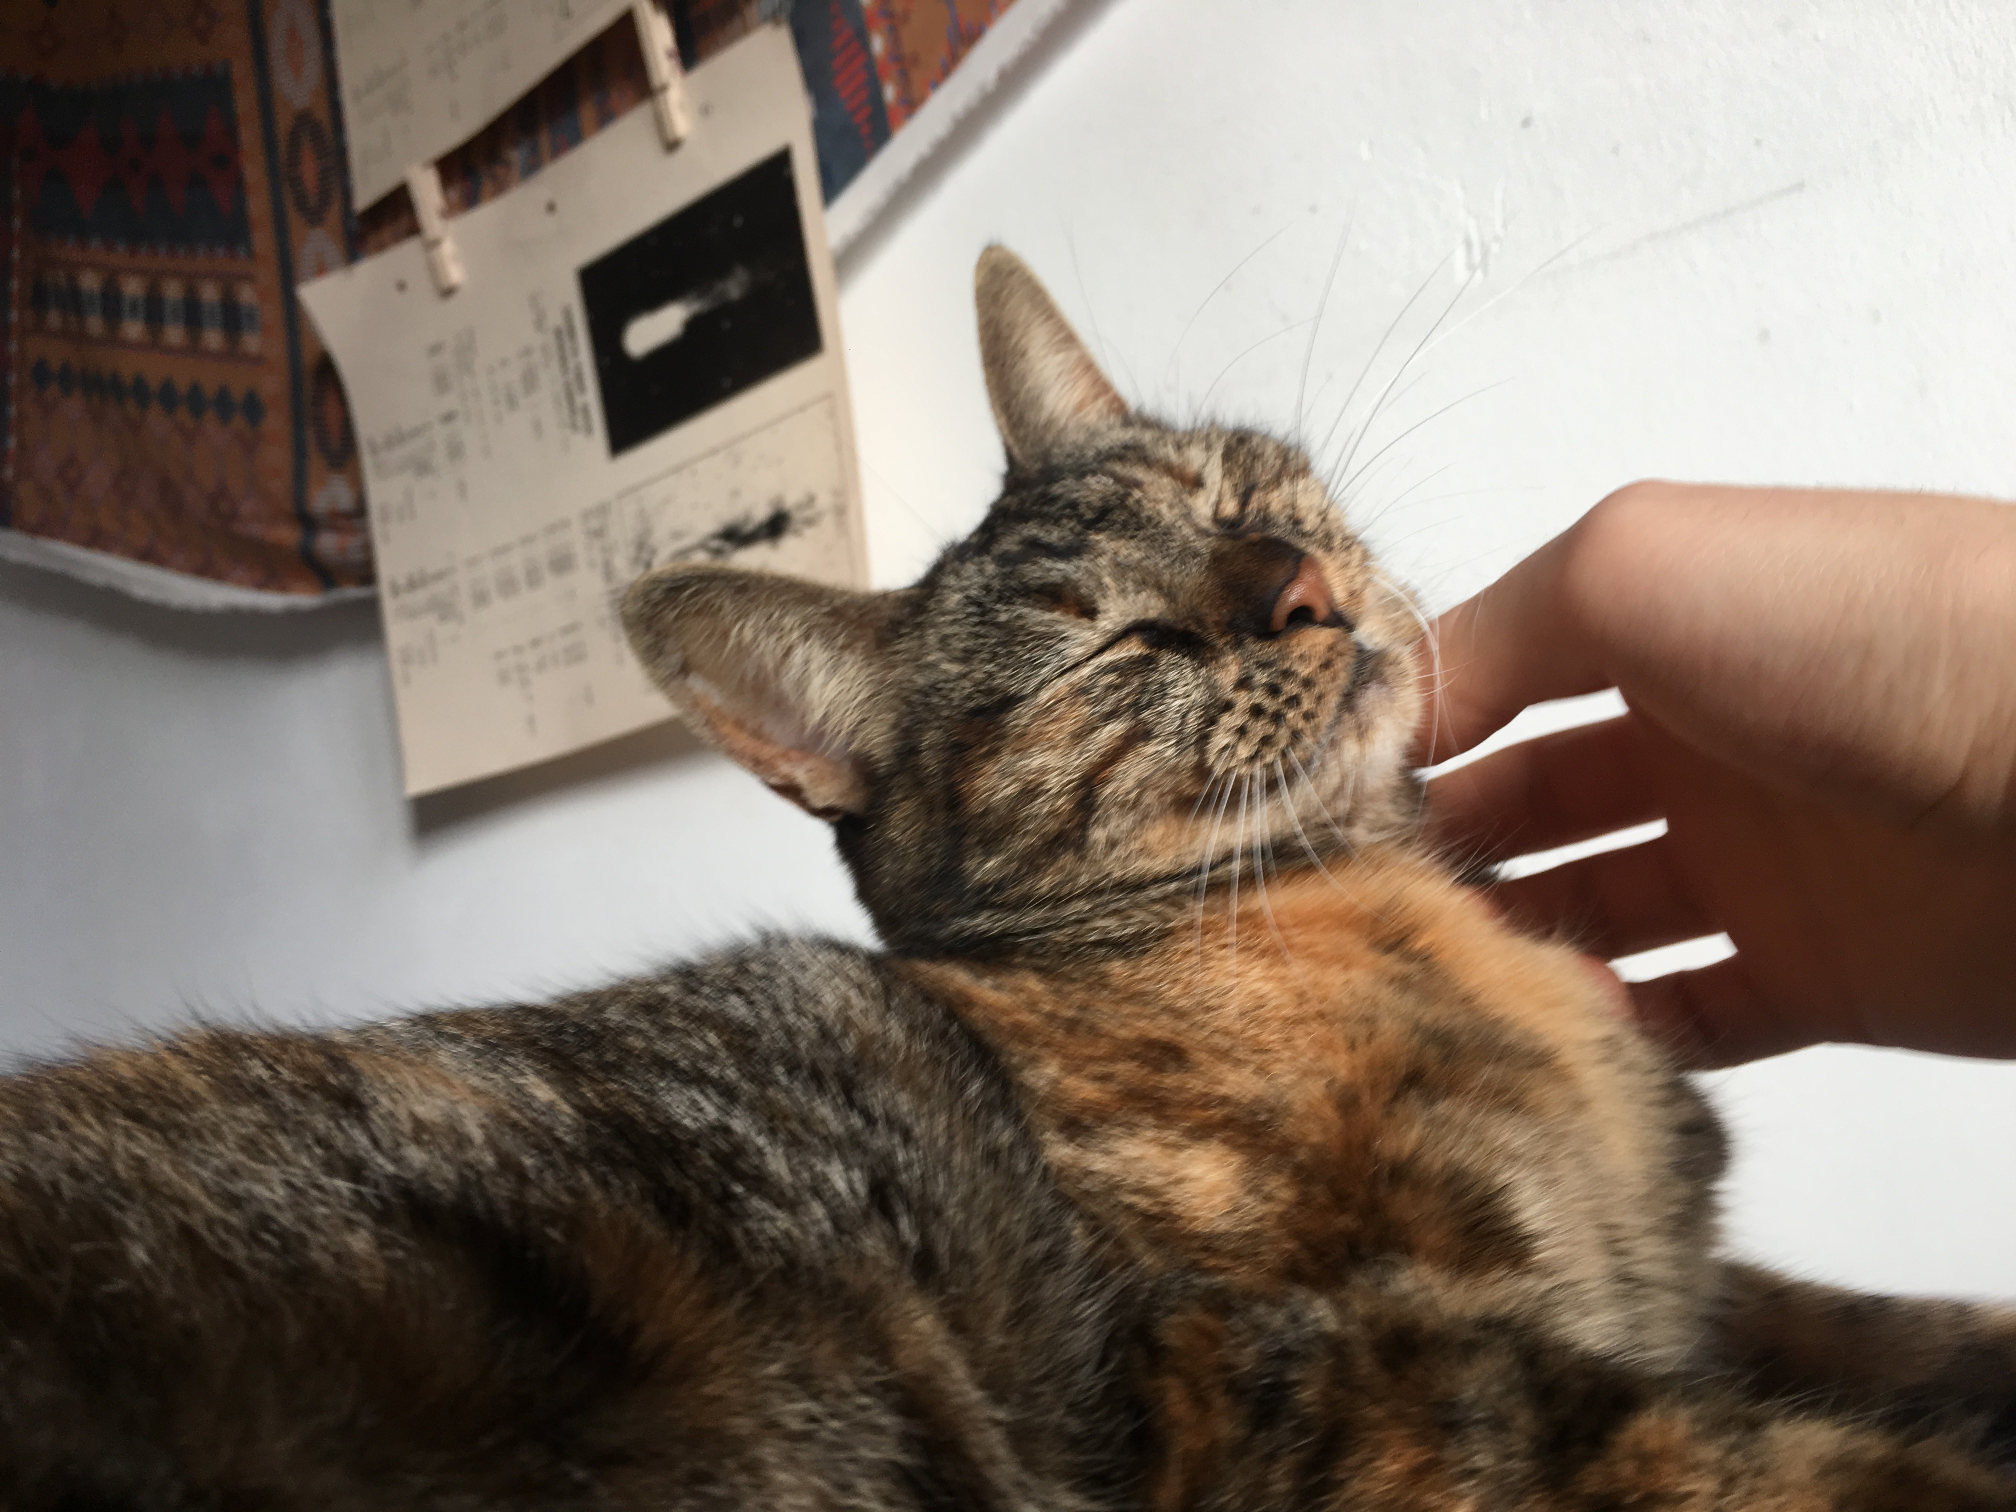
\includegraphics[width=.7\textwidth]{img/cat.jpg}
    \caption{A lief hondje.}
    \label{fig:my_label}
\end{figure}

\newpage

% Je kan zelf een referentiestijltje kiezen, 'plain' is het standaardje
% Zie:
% https://www.overleaf.com/learn/latex/Bibtex_bibliography_styles
% 
% We gebruiken het package-je 'babelbib' om de referentietjes in het nederlands te geven. Voeg daarom het woordje 'bab' toe aan het beginnetje van het stijltje.
% De optietjes zijn: babplain, babunsrt, bababbrv en babalpha.

% Het gebruiken van babplain geeft een warninkje: "BibTeX empty language in ...". Dit kan je vermijden door ",language={dutch}" toe te voegen aan elk itempje van references.bib.

\bibliographystyle{babplain}
\bibliography{references.bib}

\end{document}

% Veel succes!

% groetjes van Fons